\documentclass[min10,12pt,english]{jsbook}
\usepackage{pethesis}
\usepackage[T1]{fontenc}
%\usepackage[utf8]{inputenc}
% \usepackage{mokuji}
% \usepackage{natbib}
% \setlength{\bibsep}{12pt}
%\input GoudyIn.fd
%\newcommand*\initfamily{\usefont{U}{GoudyIn}{xl}{n}}
% \usepackage{libertine}
% \usepackage{Typocaps}
% \usepackage{lettrine}

%\usepackage[dvipsnames]{xcolor}
% \renewcommand{\LettrineFontHook}{\color{BrickRed}\Typocapsfamily{}}
% \setcounter{DefaultLines}{3}
\usepackage{lettrine}
\usepackage{Typocaps}
% lettrine formatting
\renewcommand{\LettrineFontHook}{\Typocapsfamily{}}
\setlength{\DefaultNindent}{0em}
\setcounter{DefaultLines}{3}
%\input GoudyIn.fd
%\newcommand*\initfamily{\usefont{U}{GoudyIn}{xl}{n}}
%%%%%%%%%%%%%%%%%%%%%%%%%%%%%%%%%%%%%%%%%%%%%%%%%%%%%%%%%%%%%%%%%%%%%%%
%%%%%%%%%%%%%%%%%%%%%%%%%~PACKAGES~%%%%%%%%%%%%%%%%%%%%%%%%%%%%%%%%%%%%
%%%%%%% MATH
\usepackage{amsmath,amssymb,bm}
\usepackage{mathtools}
\usepackage{amsfonts}
\usepackage{amsthm}
\usepackage{arydshln}
%
%\usepackage{cite}
%

\usepackage{mediabb}
\usepackage{caption}
\usepackage{tabularx}
\usepackage{float}
%\usepackage{symbol}{footmisc}
\usepackage{epsfig}
\usepackage{graphicx}
\usepackage{subfigure}
\usepackage{mdwlist}
%\usepackage{subcaption}

\graphicspath{{Figures/}}

\DeclareGraphicsRule{.png}{eps}{.xbb}{}
\DeclareGraphicsRule{.jpg}{eps}{.xbb}{}
\usepackage{grfext}
\AppendGraphicsExtensions*{.png,.jpg}
\usepackage{tikz}
\usetikzlibrary{shadows,shapes,arrows,fit,calc,patterns,decorations.pathmorphing,decorations.markings,positioning,backgrounds}
\renewcommand{\rmdefault}{ptm}
\tikzset{
  basic box/.style = {
    shape = rectangle,
    align = center,
    draw  = #1,
    fill  = #1!25,
    rounded corners},
  header node/.style = {
    Minimum Width = header nodes,
    font          = \strut\Large\ttfamily,
    text depth    = +0pt,
    fill          = white,
    draw},
  header/.style = {%
    inner ysep = +1.5em,
    append after command = {
      \pgfextra{\let\TikZlastnode\tikzlastnode}
      node [header node] (header-\TikZlastnode) at (\TikZlastnode.north) {#1}
      node [span = (\TikZlastnode)(header-\TikZlastnode)]
        at (fit bounding box) (h-\TikZlastnode) {}
    }
  },
  hv/.style = {to path = {-|(\tikztotarget)\tikztonodes}},
  vh/.style = {to path = {|-(\tikztotarget)\tikztonodes}},
  fat blue line/.style = {ultra thick, blue}
}
%
\usepackage{pgfplots} 
\usepgfplotslibrary{groupplots}
\usepgfplotslibrary{patchplots}
\pgfplotsset{
	compat=1.14,
	colormap={no data}{
		color=(white)
		%        color=(white)
		color=(red)
	},
	colormap/bluered,
	colormap={parula}{
		rgb255=(53,42,135)
		rgb255=(15,92,221)
		rgb255=(18,125,216)
		rgb255=(7,156,207)
		rgb255=(21,177,180)
		rgb255=(89,189,140)
		rgb255=(165,190,107)
		rgb255=(225,185,82)
		rgb255=(252,206,46)
		rgb255=(249,251,14)
	},
}
% and optionally (as of Pgfplots 1.3): 
\pgfplotsset{compat=newest} 
\pgfplotsset{plot coordinates/math parser=false} 

\usepackage{minitoc}
\usepackage{hhline}
\usepackage{slashbox}
\usepackage{booktabs}
%\usepackage[usenames]{color}
\usepackage{colortbl}
\usepackage{braket}
\usepackage{bm}
\usepackage{otf}
\usepackage{xcolor}

%\usepackage[LGR,T1]{fontenc}
%\newcommand{\textgreek}[1]{\begingroup\fontencoding{LGR}\selectfont#1\endgroup}

\usepackage{titletoc}
\usepackage{algorithm}
\usepackage[noend]{algpseudocode}
\usepackage{makecell} % for change line inside a table cell (added by Jiang)
\usepackage[nomath,nosf,notextcomp]{kpfonts}
\usepackage{fourier}\selectfont
\usepackage[bb=boondox,bbscaled=.95]{mathalfa}\selectfont
\makeatletter
\def\BState{\State\hskip-\ALG@thistlm}
\makeatother

\usepackage{calrsfs}
\DeclareMathAlphabet{\pazocal}{OMS}{zplm}{m}{n}
%
\newcommand{\Lb}{\pazocal{H}}
% modify the space of chapter name by Jiang
% the values of the distance need to be improved to get better alignment
\titlecontents{chapter}[2cm]{\addvspace{2pt}\bfseries}{\hspace*{2pt}\contentslabel[\thecontentslabel]{5.7em}}{\hspace*{-5.45em}} 
{\titlerule*[4pt]{.}\contentspage}
% for more info:
% https://tex.stackexchange.com/questions/130670/separation-between-label-and-title
% http://mirror.switch.ch/ftp/mirror/tex/macros/latex/contrib/titlesec/titlesec.pdf

\titlecontents{section}[2.5em]{}
  {\hspace{1em}\contentslabel{2.5em}}%change the argument to obtain the 
                         %desired spacing
  {\hspace*{-2.3em}}
  {\titlerule*[4pt]{.}\contentspage}
  
\titlecontents{subsection}[2.5em]{}
  {\hspace{3.5em}\contentslabel{2.5em}}%change the argument to obtain the 
                         %desired spacing
  {\hspace*{-2.3em}}
  {\titlerule*[4pt]{.}\contentspage}

\titlecontents{figure}[3.5em]{}
  {\contentslabel{3.5em}}%change the argument to obtain the 
                         %desired spacing
  {\hspace*{-2.3em}}
  {\titlerule*[4pt]{.}\contentspage}

\titlecontents{table}[3.5em]{}
  {\contentslabel{3.5em}}%change the argument to obtain the 
                         %desired spacing
  {\hspace*{-2.3em}}
  {\titlerule*[4pt]{.}\contentspage}  
  
  
%\renewcommand{\mtctitle}{}
\setlength{\mtcindent}{6pt} % minitocのインデントを小さく
\renewcommand{\mtcSfont}{\normalsize\rm} % minitocのsection用フォント
\renewcommand{\mtcSSfont}{\normalsize\rm} % minitocのsubsection用フォント
\newcommand{\argmax}{\mathop{\rm arg~max}\limits} %argmax定義

\allowdisplaybreaks
%%%%%%%%%%%%%%%%%%%%%%%%%%%%%%%%%%%%%%%%%%%%%%%%%%%%%%%%%%%%%%%%%%%%%%%%%%%%%%%%%%%%%%%%%%%%
%%%%%%%%%%%%%%%%%%%%%%%%%%%%%%%%%%% My Commands %%%%%%%%%%%%%%%%%%%%%%%%%%%%%%%%%%%%%%%%%%%
%%%%%%%%%%%%%%%%%%%%%%%%%%%%%%%%%%%%%%%%%%%%%%%%%%%%%%%%%%%%%%%%%%%%%%%%%%%%%%%%%%%%%%%%%%%%
\newcommand{\R}{\mathbb{R}}

% operators
\newcommand{\rank}{\text{rank}}
\newcommand{\Span}{\text{span}}
\DeclareMathOperator{\conv}{conv}
\DeclareMathOperator{\diag}{diag}
\DeclareMathOperator{\Null}{null}
\DeclareMathOperator*{\argmin}{arg\,min}
% bold letters
\newcommand{\x}{\mathbf{x}}
\newcommand{\q}{\mathbf{q}}
\newcommand{\p}{\mathbf{p}}
\newcommand{\xb}{\mathbf{x}}
\newcommand{\ub}{\mathbf{u}}
\newcommand{\yb}{\mathbf{y}}
\newcommand{\Jb}{\mathbf{J}}
\newcommand{\Rb}{\mathbf{R}}
\newcommand{\Gb}{\mathbf{G}}
% cal letters
\newcommand{\Ha}{\pazocal{H}}
\newcommand{\U}{\pazocal{U}}
\newcommand{\Y}{\pazocal{Y}}
\newcommand{\X}{\pazocal{X}}
\newcommand{\La}{\pazocal{L}}
\newcommand{\A}{\pazocal{A}}
\newcommand{\C}{\pazocal{C}}
\newcommand{\M}{\pazocal{M}}
\newcommand{\V}{\pazocal{V}}
\newcommand{\Q}{\pazocal{Q}}
\newcommand{\K}{\pazocal{K}}
\newcommand{\D}{\pazocal{D}}
%\newcommand{\O}{\pazocal{O}}
%
\DeclareMathAlphabet{\mymathbb}{U}{BOONDOX-ds}{m}{n}
%
\newcommand{\TODO}[1]{\par\noindent\colorbox{red}{\parbox{\dimexpr\textwidth-2\fboxsep\relax}{\textcolor{white}{\textbf{TO DO: {#1}}}}}}
\newcommand{\mysubcaption}[1]{\begin{minipage}{\columnwidth}\begin{center}\small{#1}\end{center}\end{minipage}}
\newtheorem{thm}{Theorem}[section]
\newtheorem{cor}[thm]{Corollary}
\newtheorem{lem}[thm]{Lemma}
\newtheorem{claim}[thm]{Claim}
\newtheorem{axiom}[thm]{Axiom}
\newtheorem{conj}[thm]{Conjecture}
\newtheorem{fact}[thm]{Fact}
\newtheorem{hypo}[thm]{Hypothesis}
\newtheorem{assum}[thm]{Assumption}
\newtheorem{prop}[thm]{Proposition}
\newtheorem{crit}[thm]{Criterion}
%\theoremstyle{definition}
\newtheorem{defn}[thm]{Definition}
\newtheorem{exmp}[thm]{Example}
\newtheorem{rem}[thm]{Remark}
\newtheorem{prob}[thm]{Problem}
\newtheorem{prin}[thm]{Principle}
%\newtheorem{alg}{Algorithm}
%\newtheorem{note}{Note}
\newtheorem{summ}{Summary}
\newtheorem{case}{Case}
%
\newtheorem{rmk}[thm]{Remark}

% 図と図の間のスペース
%\addtolength\floatsep{5truemm}
% 本文と図の間のスペース
\addtolength\textfloatsep{5truemm}
% 本文中の図のスペース
%\addtolength\intextsep{0pt}
% 図とキャプションの間のスペース
%\addtolength\abovecaptionskip{5truemm}
%\usepackage[citecolor=blue]{hyperref}
%
% 論文の表紙の項目
%
\thesistype{平成31年度 修士論文}
\title{Hybrid Port--Hamiltonian Systems:\\Application to Robotics}
\etitle{ハイブリッド・ポート・ハミルトン系:ロボット応用}
\affiliation{Department of Precision Engineering, Graduate School of Engineering\\ \vspace{5pt} The University of Tokyo}%{東京大学 工学系研究科 精密工学専攻}
\supervisor{Professor Hajime Asama \\  淺間一教授}
\studentid{37-175037}
\author{Massaroli Stefano\\ マッサロリ ステファノ}
\begin{document}
\dominitoc
%表紙
\maketitle
%概要
\thispagestyle{empty}
% TITLE PAGE
\frontmatter
% ABSTRACT
\chapter*{Abstract}
\label{abst}

%%%%%%%%%%%%%%%%%%%%%%%%%%%%%%%%%%%%%%%%%%%%%%%%%%%%%%%%%%%%%%%%%%%%%%%%%%%%%%%
Accurate and robust control of robots in highly dynamic tasks is arguably one of the hardest open problems in robotics. The incapability of robots to safely and reliably interact with their environment is what still refrain them from becoming ubiquitous in our society.
%
The main challenge is due to the \textit{nonsmooth} nature of such dynamic tasks, as they often involve impacts between parts of the robot and its environment. Examples are \textit{legged locomotion}, \textit{non--prehensile} manipulation or aerial robot landing.
%
\newline

%
This issue in robotics is a fundamental control challenge, extremely appealing for the research community, which is trying to fulfill the needs of industries who are seeking more autonomy for commercial robots.
This interest expands swiftly to a theoretical level once the problem is formalized. Discontinuities of any sort used to be sworn enemies of most control theorists. However, in recent years, a new emerging field of control theory: the \textit{hybrid dynamical systems}, promises a complete set of mathematical tools to deal with tasks characterized by interacting continuous and discrete time dynamics. Besides, this framework is by no means close to solve the robotics problem. Control theorists often spend too much time on over--complicated math without foresight of its applications. 
\newline

%
Nevertheless, the work presented in this thesis hinges on the most fundamental concept of classical and modern physics: \textit{energy}. Energy is the key to understand, and thus control, the behavior of dynamical system by physical insights. The most relevant mathematical tool in this context is the one of \textit{port--Hamiltonian systems}. The aim of this thesis is to provide a unified modeling framework merging the ones of port--Hamiltonian and hybrid systems through consistent and practically useful results.
%
\newline

%
The research work embraces four different objectives: 
characterize a new unified modeling strategy to tackle highly dynamic robotic tasks; apply the theory to cope with the challenging \textit{ball--dribbling robot} problem; show the broad applications' spectrum of the developed framework by adopting it into to bear pure control theory problem; perform a first step towards real implementation of such control systems through system identification task.
%
\newline

%
The contribution of this thesis is primarily theoretical, however, all chapters are application--oriented displaying real examples with simulations.


%Accurate localization and mapping are very important for mobile robots working in indoor environments where human exists. In order to localize and map accurately, a rangefinder (LRF) is widely used because of it high accuracy in distance measuring. In modern indoor environments, glass is very common. However, glass is usually not shown on the map correctly when using LRF, because it cannot be detected by LRF from all angles, as other objects. The incorrect map brings the danger of crashing into the glass to the mobile robot when path planning. Furthermore, the limited ability of LRF in glass detection negatively influences the localization accuracy of the mobile robots. 
%
%To solve the problems mentioned above, this thesis proposes to build a glass confidence map which can show all objects on the map, glass included, and their probability of being glass. The purpose of this thesis is to build such a glass confidence map. The method proposed is to first classify glass and non-glass objects, and then process them differently in order to get a better map. 
%
%%The reason glass need to be processed differently is because in standard mapping stage, objects are assumed to be detectable from all incident angles, while glass does not match this assumption. 
%
%To classify the glass and non-glass objects, a neural network based classifier is proposed, with LRF's measured intensities, distances and incident angles as inputs, as well as glass probability as output. The classification method is based on the assumption proposed in this thesis, that the LRF's measured intensity is mainly influenced by material features, incident angle and distance, and therefore material features can be inferred by LRF intensity, distance and incident angle. To verified the assumption, experiments are performed, and the results show glass and non-glass panels have obviously different patterns and are separable in the feature space of intensity, distance and incident angle. The proposed neural network classifier has 2 hidden layers, 10 nodes in each hidden layer, and is trained and tested using experimental data. 
%
%Additionally, a novel map building method is proposed to build the targeted glass confidence map using the glass probability and information from standard Simultaneous Localization and Mapping (SLAM). First, the glass probability is registered to a temporary map, using a Gaussian Filter to reduce the influence of uncertainty in robot pose and LRF measurements. Second, to remove noise, the temporary map is filtered based on both occupancy probability and glass probability. Glass objects are applied to a lower occupancy threshold than non-glass objects, considering the fact glass cannot be detected consistently by the LRF.
%
%To verify the proposed method, two experiments in two different environments are performed. As a result, glass confidence maps are built, with more glass shown correctly than maps built by standard methods. Besides, quantitative analysis on the results shows that the neural network classifier classify glass and non-glass objects with high accuracy. In summary, the proposed method can build glass confidence maps successfully and accurately.

\clearpage
%%%%%%%%%%%%%%%%%%%%%%%%%%%%%%%%%%%%%%%%%%%%%%%%%%%%%%%%%%%%%%%%%%%%%%%%%%%%%%%
%%% Local Variables:
%%% mode: katex
%%% TeX-master: "../thesis"
%%% End:

%目次
\tableofcontents
%図目次
\listoffigures
%表目次
\listoftables

\chapter*{Notations, Symbols and Acronyms}
\label{symbols_notations}

Matrices are capitalized and in bold font, vectors are in bold font and scalars are in italic font; unless specifically noted.
\mbox{}\\
\mbox{}\\
\begin{tabularx}{0.95\textwidth}{p{2.75cm} X}
 \textbf{Notations} 	&\textbf{Meaning}\\
 $x$                    & scalar\\
 $\xb$                  & vector\\
 $\mathbf{X}$           & matrix\\
 $\X$                   & set\\
 $\xb_i$                &$i$-th element of $\xb$\\
 $\mathbf{X}_{ij}$      &entry of $\mathbf{X}$ corresponding to the $i$-th row and $j$-th column\\
 $\succ,\prec,\succeq,\preceq$ & symbols used in matrix inequalities\\
 $(\mathbf{v},\mathbf{w})$ & given two vectors $\mathbf{v}$ and $\mathbf{w}$,  $(\mathbf{v},\mathbf{w})\triangleq \left[\mathbf{v}^\top,\mathbf{w}^\top\right]^\top$ \\
 $\dot{x}$                   &time derivative of the variable $x$, $\dot{x}\triangleq\dfrac{dx}{dt}$\\
 $x^+$                  &next value of the quantity $x$ after a discrete--time event
\end{tabularx}

\mbox{}\\
\mbox{}\\
\begin{tabularx}{0.95\textwidth}{p{2.75cm} X}
\textbf{Symbols} 			& \textbf{Meaning}\\
 $\R$                       & Set of Reals\\
 $\mathbb{N}$               & Set of Naturals\\
 $\R^+$                     & Nonnegative reals\\
 $\mathbb{N}_{\leq s}$      & Naturals less than $s$\\
 $\mathbb{N}^*$             & Naturals without the zero element\\
 $\mathbb{I}_n$             & $n$ by $n$ identity matrix\\
 $\mathbb{O}_n$             & $n$ by $n$ zero matrix\\
 $\mathbb{O}_{n\times m}$   & $n$ by $m$ zero matrix\\
 $\mymathbb{0}_n$           & origin of $\R^n$\\
 $\mathbb{1}_n$             & unitary vector of $\R^n$\\
 $\La_2^m$                  & set of square--integrable functions $z:\R\rightarrow\R^m$\\
 $\langle \cdot,\cdot\rangle$ & {inner product of $\R^n$. $\langle \cdot,\cdot\rangle:\R^n\times\R^n\rightarrow\R$.\newline Let $\mathbf{v},~\mathbf{w}\in\R^n$, $\langle \mathbf{v},\mathbf{w}\rangle = \mathbf{v}^\top \mathbf{w}$} \\
 $\|\cdot\|_2$              & induced norm of $\R^n$. Let $\mathbf{v}\in\R^n$, $\|\cdot\|_2\triangleq\sqrt{\langle \mathbf{v},\mathbf{v}\rangle}$ \\
 $\|\cdot\|_\infty$         & infinity norm\\
 $\bm\nabla\Ha(\xb)$        & Given a scalar--valued function $\Ha:\R^n\supseteq\X\rightarrow\R$, $\bm\nabla\Ha(\xb)$ denotes its transposed gradient, i.e. $\bm\nabla\Ha(\xb):\X\rightarrow\R^n$ such that $\bm\nabla\Ha(\xb)\triangleq\left(\dfrac{\partial \Ha}{\partial\xb}\right)^\top$\\
 $\bm\nabla^2\Ha(\xb)$      & Hessian matrix of $\Ha$, i.e. $\bm\nabla^2\Ha(\xb):\X\rightarrow\R^{n\times n}$ such that $\bm\nabla^2\Ha(\xb)\triangleq\dfrac{\partial}{\partial\xb}\dfrac{\partial\Ha}{\partial\x}$\\
 $\conv(\Lambda)$           & convex hull of a finite subset $\Lambda\subset\R^n$ defined by the convex combinations of its elements. 
\end{tabularx}

\mbox{}\\
\mbox{}\\
\begin{tabularx}{0.95\textwidth}{p{2.75cm} X}
 \textbf{Acronyms} 			& \textbf{Meaning}\\
% % MCL
PH				    & Port--Hamiltonian\\
HDS					& Hybrid Dynamical System\\
\end{tabularx}


%\clearpage
%\begin{center}
%    \textgreek{L'aje bi'wsas}
%\end{center}
%Epicurus

\mainmatter

%
\chapter{{Introduction}}
\label{chap:introduction}
\minitoc

\thispagestyle{empty}

\newpage
%%%%%%%%%%%%%%%%%%%%%%%%%%%%%%%%%%%%%%%%%%%%%%%%%%%%%%%%%%%%%%%%%%%%%%%%%%%%%%

%\section{Motivation}

%\clearpage

\section{Background}
\definecolor{brickred}{rgb}{0.8, 0.25, 0.33}
\lettrine[lines=4]{\color{brickred}M}{odelling} , analysis and control of \textit{nonsmooth} systems is an interesting and open problem which attracts the attention of a wide range of researchers, from physicists and mechanical engineers to specialists in control and automation~\citep{brogliato1999nonsmooth,stronge2018impact}.
The interaction between continuous and discrete-time dynamics arises, for instance, while considering the behavior of a mechanical system in presence of impacts: its dynamics cannot be represented only by means of differential equations. The theory of~\textit{hybrid dynamical systems} (HDS) is the formalism in which this type of models can be described. Overviews of this framework are given in~\citep{van2000introduction,haddad2006impulsive}. In particular, the most general and recent modeling approach is the one of \textit{hybrid inclusions} developed in recent years \citep{goebel2009hybrid}. This field of Automatic Controls generally investigates systems characterized by the interaction of continuous and discrete time dynamics as well as by multimodality \citep{Goebel2012}.
%
\newline

%
%%%%%%%%%%%%%%%%%%%%%%%%%%%%%%%%%%%%%%%%%%%%%%%%
%\subsection{The Manipulation Problem for Highly Dynamic Tasks}
%\subsection{The Role of Energy in Robot Control}
In the last three decades, the fundamental concept of \textit{energy} experienced an impressive growth process in engineering practice and in particular in system theory. 
%
%\newline
%
%
The framework of \textit{passivity--based control} (PBC) is now a well--established branch of nonlinear control theory and aims at treating dynamical systems as devices able to exchange energy, rather than to process signals \citep{ortega2001putting}. 
This is possible by equipping dynamical systems with additional structure (e.g. storage functions, supply rates, etc.) by means of which the concepts of energy and input/output characterization of the system are connected in a unique framework \citep{sontag2008input}.
%
\newline

%
In this context, another fundamental paradigm regards the \textit{interconnection} of systems by means of \textit{power ports} \citep{duindam2009modeling}, which led to the definition of \textit{port-Hamiltonian systems} \citep{MASCHKE1992359,ortega2001putting,van2014port}, the mathematical framework in which PBC developed naturally, merging geometry and network theory. Hence, the control problem reduces to the design of a dynamical system (the controller) and an interconnection structure that ``shapes'', in a desired way, the energy of the original system \citep{ortega2001putting,ortega2008control}.
%
%\newline
%
%
This approach allows control engineers to pay particular attention to the performance of the control system and not only to stabilizability (as common in nonlinear control).
%
%\newline
%
%
In classic robot control, the theory of passivity lead to several successful approaches, such as the \textit{gravity--compensation} \citep{arimoto1984stability} and \textit{impedance} controller \citep{secchi2007control}. Other interesting application are robots with flexible links \citep{macchelli2009} and elastic joints \citep{zhang2016}.
%
%%%%%%%%%%%%%%%%%%%%%%%%%%%%%%%%%%%%%%%%%%%%%%%%%%%%%%%
\subsection{Energy as Common Factor Among Interactions}\label{subsec:comm_fact}
%
Driven by a physical intuition, it is rather straightforward to recognize energy as the \textit{lingua franca} between different physical domains. This idea lead, in the early sixties, H. Paynter to establish the field of \textit{port--based modeling} \citep{paynter1961analysis}.
%
\newline

%
A physical system, in fact, may exhibit a \textit{dynamical behavior} if and only if some energy exchange happen within its \textit{internal structure} (components) or with the external world. In any physical domain there exists pair of dual variables (see Appendix A) often called \textit{flows} and \textit{efforts} which intrinsically form \textit{power ports}, interfaces through which energy flows \citep{secchi2007control}. Table \ref{tab:ef} lists the effort and flow variables for several physical domains.
%
\begin{table}[t]
	\centering
	\caption{Efforts and flows variables for various physical domains.}
	\begin{tabular}{|c|cc|cc|} \hline
			\rowcolor{gray!50}\textbf{Domain}&{\centering \textbf{Effort}}&&{\centering \textbf{Flow}}&\\\hline
			Mechanics (translational)&Force&$F$&Velocity&$v$\\\hline
			\rowcolor{gray!15}Mechanics (rotational)&Torque &$\tau$&Angular Velocity &$\omega$\\\hline
			Electric&Voltage &$v$&Current &$i$\\\hline
			\rowcolor{gray!15}Hydraulic&Pressure& $p$&Volume Flow &$Q$\\\hline
			Thermodynamic&Temperature &$T$&Entropy Flow &$\dot{E}$\\\hline
	\end{tabular}
	\label{tab:ef}
\end{table}
%
\newline

In robot manipulation, this description of dynamical phenomena may result particularly useful to model the interaction between the robot end--effector and the object, which indeed exchange energy with each other in a continuous fashion.
%
In fact, the port--Hamiltonian framework allows to explicitly capture the physical phenomena behind this continuous interaction. Furthermore, in this perspective, the robot controller can also be thought as an other dynamical system interconnected with the robot and exchanging energy with it. 
This approach results to be both, general and versatile.
%
The theory of passivity--based control of port--Hamiltonian system has been already successfully applied in a variety of manipulation tasks: from grasping \citep{stramigioli99} and soft--finger manipulation \citep{ficuciello2010} to non--prehensile tasks, e.g. object rolling \citep{donaire2017,serra2019}.
%
\newline

%
Besides, when the robot tasks involve \textit{nonsmooth} phenomena such as mechanical impacts or dynamic friction \citep{brogliato1999nonsmooth}, the classical passivity--based techniques cease to work due to the discontinuities in system's state along trajectories. 

However it can be noticed that energy is the undisputed protagonist also of this type on discrete (instantaneous) interactions. Thus, an energy--based reasoning might be carried out to overcome the challenges given by the hybrid nature of these robot tasks.  

From now on, we will refer to any robotic tasks which is hybrid in nature, i.e. it includes interacting continuous and discrete phenomena, as \textit{highly dynamic tasks}.
%%%%%%%%%%%%%%%%%%%%%%%%%%%%%%%%%%%%%%%%%%%%%%%%%%%%%%%%%%%%%%%%%%%%%
%\subsection{Hybrid port--Hamiltonian System: a New Tool For Robotics}
\subsection{Research Problem: Control Highly Dynamic Robotic Tasks}
%
The extension of passivity--based control of port--Hamiltonian systems to the hybrid case is highly desirable. In fact, this will allow to establish a new general and unified framework to model and control robots performing highly dynamic tasks.
%
\newline

%
Examples of these tasks in the manipulation context are:
ball--juggling \citep{sanfelice2007hybrid, tian2013}, ball--dribbling \citep{Batz2010, haddadin2018exploiting} or even tossing/catching of a deformable object \citep{ruggero2018}. 
Other hybrid tasks may be related to \textit{self manipulation}, e.g. dynamic walking \citep{spong2007,westervelt2018feedback}, hopping robots \citep{Ishikawa2003} and control of powered exoskeletons \citep{harib2018feedback,lv2018design}. The one--dimensional version of the ball--juggling and ball--dribbling systems are represented in Fig. \ref{fig:1D}.
%
\newline

%
One of the most clear proofs of the necessity of an novel unified framework merging energy--based approaches to hybrid systems is given by all the research work present in literature: although they belong to the same class of robot control problems, each tasks is solved with \textit{ad--hoc} solutions, without any analysis of a bigger picture.  
%
\newline

Furthermore, as underlined in Subsection \ref{subsec:comm_fact}, the span of validity of this new general framework could indeed be extended to any physical domain, and thus employed to find potential solutions in different branches of engineering.
%
\begin{figure}[!h]
	\centering
	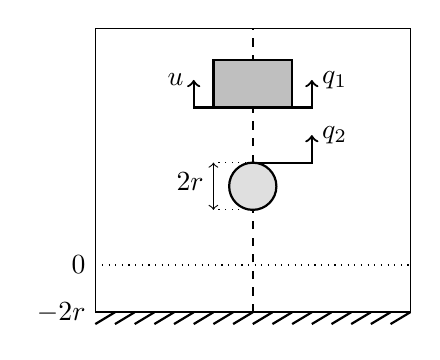
\begin{tikzpicture}
	%
	% axes
	\draw[thick] (0,-0.6)--(4,-0.6);
	\draw[dotted] (0,0) node[anchor = east] {\color{black}$0$}--(4,0);
	\draw[thick,dashed] (2,-0.6) -- (2,3);
	\draw (0,-0.6) node[anchor = east] {$-2r$} -- (4,-0.6) -- (4,3) -- (0,3) -- (0,-0.6);
	
	% robot
	\fill[gray!50, draw = black,thick] (1.5,2) rectangle (2.5,2.6);
	% ball
	\fill[gray!25, draw=black,thick] (2,1) circle (0.3);
	%	
	\draw[thick,->] (2.5,2) -- (2.75,2) -- (2.75,2.35) node[anchor=west] {$q_1$};
	\draw[thick,->] (1.5,2) -- (1.25,2) -- (1.25,2.35) node[anchor=east] {$u$};
	\draw[thick,->] (2,1.3) -- (2.75,1.3) -- (2.75,1.65) node[anchor=west] {$q_2$};
	%
	\draw[dotted] (2,1.3) -- (1.5,1.3);
	\draw[dotted] (2,0.7) -- (1.5,0.7);
	\draw[<->] (1.5,0.7) -- (1.5,1.3)  node[anchor=north east] {$2r$};
	%
	\foreach \x in {0,0.25,0.5,0.75,1,1.25,1.5,1.75,2,2.25,2.5,2.75,3,3.25,3.5,3.75}
	\draw[thick] (\x,-0.75) -- (\x+0.25,-0.6);
\end{tikzpicture}
	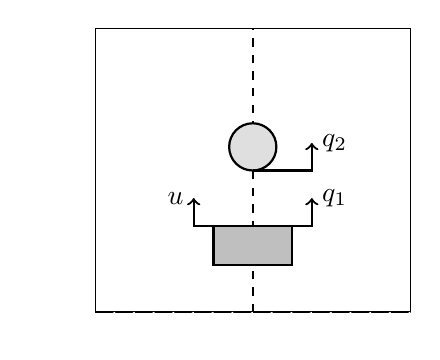
\begin{tikzpicture}
	%
	\draw[thick] (0,-0.6)--(4,-0.6);
	\draw[thick,dashed] (2,-0.6) -- (2,3);
	\draw (0,-0.6)  node[anchor = east] {\color{white}$-2r$} -- (4,-0.6) -- (4,3) -- (0,3) -- (0,-0.6);
	
	% robot
	\fill[gray!50, draw = black,thick] (1.5,0) rectangle (2.5,0.5);
	% ball
	\fill[gray!25, draw=black,thick] (2,1.5) circle (0.3);
	%	
	\draw[thick,->] (2.5,0.5) -- (2.75,0.5) -- (2.75,0.85) node[anchor=west] {$q_1$};
	\draw[thick,->] (1.5,0.5) -- (1.25,0.5) -- (1.25,0.85) node[anchor=east] {$u$};
	\draw[thick,->] (2,1.2) -- (2.75,1.2) -- (2.75,1.55) node[anchor=west] {$q_2$};
	\foreach \x in {0,0.25,0.5,0.75,1,1.25,1.5,1.75,2,2.25,2.5,2.75,3,3.25,3.5,3.75}
	\draw[color = white] (\x,-0.755) -- (\x+0.25,-0.6);
\end{tikzpicture}
	\caption[One--dimensional ball--dribbling and ball--juggling robotic systems.]{One--dimensional ball--dribbling (left) and ball--juggling (right) robotic systems. The position of the robot (rectangle), is represented by the variable $q_1$ while $u$ is an input force applied to it. The position of the ball (circle), of radius $r$, is represented by $q_2$. The ball--juggling system presents a single impact, i.e. the one between the robot and the ball. The ball--dribbling system, instead, is characterized by two impacts: ball--robot and ball--ground.}
	\label{fig:1D}
	%
\end{figure}
%
%%%%%%%%%%%%%%%%%%%%%%%%%%%%%%%%%%
\subsection{Beyond Robot Control}
It has been proven that a novel unified framework for controlling highly dynamic robotic tasks is needed but cannot be approached in a systematic general way due to the \textit{nonsmooth} nature of the robotic tasks.
%
\newline

%
However, many control systems presents discontinuities and multimodality due to the control algorithm itself rather then physics. 
For example, a system subjected to a \textit{sliding--mode controller} \citep{pisano2011sliding} is, technically speaking, an hybrid system. Moreover, the whole framework of \textit{switching control} belongs to field of hybrid dynamical systems.
%
\newline

%
Very simple practical example of how a controller give an hybrid nature to dynamical systems, are the temperature regulator of a room or the water--level control in tanks.
%
\newline
    
%
In the light of this considerations, it is legitimate pose the following questions: \newline
\textit{Can hybrid control systems be modeled from an energetic point of view in port--Hamiltonian fashion?}\newline
\textit{If yes, which theoretical advantages would this formulation give?}

%%%%%%%%%%%%%%%%%%%%%%%%%%%%%%%%%%%%%%%
\subsection{The Identification Problem}
%
As common in Automatic Controls, controller design, simulations and diagnostics of hybrid dynamical systems require an accurate knowledge of the model. However, these {processes} are always characterized by sets of parameters which are typically not available.
%
\newline

%
System identification techniques are the interface between real world application and mathematical world of control theory and mathematical abstraction~\citep{LJUNG20101}. These methods aim to obtain estimates of the parameters and update the model from direct measurements collected during the time evolution of the system~\citep{soderstrom2018errors,SODERSTROM2019}.
%
\newline

%
Dealing with robotic systems, it is well known that inertial parameters must often be thoroughly estimated with well designed identification experiments. Moreover, if the robot experiences impacts or sudden state changes, it is intuitive to understand that further parameters given by the hybrid part of the system must also be estimated. 
Thus, in order to implement any robot controllers for highly dynamic tasks, it is necessary to solve the identification problem first.
%
\newline

%
The majority of the literature on identification of hybrid systems is related to classes of (discrete--time) Piece Wise Affine systems (PWA), i.e. systems which are defined by subdividing the  space into polyhedral regions which have associated an affine state update equation \citep{Bemporad,Ferrari,Juloski,juloski2005bayesian,Paoletti}.
% 
\newline

%
Besides, the identification of hybrid dynamical system in the form of \textit{hybrid inclusions} has to be explored yet. In fact, a systematic identification procedure for this class of systems currently is still missing. Note that, many of the robotics tasks discussed above can be modeled within this framework.
%
\newline

%
Real implementation of those tasks would undoubtedly require the knowledge of some parameters of the plant. Thus, if a novel unified modeling framework merging port--Hamiltonian and hybrid systems is proposed alongside new control techniques, the systematic estimation of physical parameters of both continuous (e.g. mass, inertia, friction) and discrete (e.g. impact restitution coefficient) parts of models  will be needed.
%
\clearpage
%%%%%%%%%%%%%%%%%%%%%%%%%%%%%%%%%%%%%%%%%%%%%%%%%%%%%%%%%%%%%%%%%%%%%%%%%%%%%%%

\section{{Aims and Objectives}}\label{sec:aim}
The aim of this thesis is to present a novel control theoretical framework for physical systems with nonsmooth and multimodal behaviors, with a special insight toward robot control tasks where the current--state--of--the--art approaches fail.

The main objectives are:
%
\begin{itemize}
    \item [1.] \textbf{to develop a novel control theoretical framework by merging the theories of port--Hamiltonian systems and hybrid systems}.
    
    With the aim of solving a robot control problem, the theory of \textit{hybrid port--Hamiltonian systems} is developed combining the theories of port--Hamiltonian systems and \textit{hybrid inclusions}, one of the most general representations of hybrid dynamical systems.
    \newline
    %
    \item [2.] \textbf{to apply the developed theory to a robot control task and prove its effective within the robotics framework}. 
    
    Considering the ball--dribbling robot problem, a novel controller, the \textit{iterative energy shaping} is systematically synthesized, proving the capabilities of the proposed framework.
    \newline
    %
    \item [3.] \textbf{to demonstrate how the developed theory goes beyond robotics and can be used to model a broad variety of control systems}. 
    
    A novel nonlinear hybrid controller for linear time--invariant system is derived from passivity--based techniques, and then this purely control theoretical problem is expressed via hybrid port--Hamiltonian systems.
    \newline
    %
    \item[4.] \textbf{to derive a new systematic identification procedure for a class of hybrid systems}.
    
    As most of hybrid control systems (including the proposed ones) require some knowledge of the physical parameters of the controlled plant, a new systematic procedure is presented to solve the estimation problem. This method can be applied to a variety of hybrid port--Hamiltonian systems 
    
    \end{itemize}
%





%
\clearpage
%%%%%%%%%%%%%%%%%%%%%%%%%%%%%%%%%%%%%%%%%%%%%%%%%%%%%%%%%%%%%%%%%%%%%%%%%%%%%%%

\section{Thesis Content and Structure}
\subsection{Thesis Outline}
This thesis is structured in seven chapters which implement the aim described in \ref{sec:aim}. 
These seven chapter can be logically clustered in four main parts: Introduction and background, theoretical results, applications and conclusions. In line with the objectives, a detailed structure of this thesis is shown in Figure \ref{fig:ThesisStructure}.
%
\newline

%
\textbf{Chapter 1} describes the main motivations, purpose and approach of this study.
%
\newline

%
\textbf{Chapter 2} briefly introduces the fields of port--Hamiltonian systems and hybrid dynamical systems. Throughout the chapter, several illustrative examples related to robotics, mathematical biology and physics are provided to highlight the practical importance of the presented theoretical concepts. 

In the first half of the chapter, the input--state--output model of a port-Hamiltonian system is derived and its most relevant properties are described. Moreover, the basic theory of the energy--balancing passivity--based control is also presented. In the second part of the chapter, the basic results on hybrid systems are introduced. In particular, it will be focused on the class of \textit{hybrid inclusions} and its stability/passivity theory.  The chapter concludes with a summary of the previous attempts to merge the two frameworks and their main limitations. 
%
\newline

%
\textbf{Chapter 3} deals with the definition and characterization of hybrid-port Hamiltonian systems. Starting from the concepts revised in the previous chapter, the new framework is here consistently developed. First, the basic assumptions are stated and the hybrid port--Hamiltonian model is derived. The concept of passivity is subsequently extended to the new model. Necessary and sufficient conditions for passivity are also reported and proved. Then, Lyapunov stability is extended from the one for hybrid inclusions. Finally, all the previous results are used to transfer to the hybrid case some of the features of passivity--based control for port--Hamiltonian systems. As for Chapter 2, application examples will be provided throughout the chapter.
%
\newline

%
\textbf{Chapter 4} introduces the first real application of the developed theory. In particular, the problem of modeling and control a ball--dribbling robot is considered. The main challenges offered by this systems are: under-actuation, dynamic decoupling between the robot and the ball and impacting interactions. First, the system is consistently modeled in hybrid port--Hamiltonian form. Then, a novel energy--based controller is derived from physical intuitions on the system. This controller enhance the classic energy shaping with the iterative learning, allowing the robot to rhythmically bounce the ball at a desired height. Simulations are performed to prove the effectiveness and robustness of the controller.   
%
\newline

%
\textbf{Chapter 5} considers the problem of controlling a linear time--invariant system with a finite number of set points. At first, a nonlinear passive controller is used to stabilize simultaneously all the desired set points. Then, a hybrid optimal impulse controller is designed to switch the between the set points. Numerical simulations are carried out for a mechanical system, proving the results. Alongside the theoretical relevance of the developed control technique, it is finally shown how the controlled system can be modeled as hybrid port--Hamiltonian system, implicitly inheriting some useful properties to analyze its behaviour.
%
\newline

%
\textbf{Chapter 6} proposes a new systematic approach for the identification of a class of hybrid dynamical systems. The main challenge offered by the considered class of systems is the detection of state discontinuities from a time series of state measurements. The proposed solution is based on the analytical computation of an upper bound on the numerically computed time--derivative of the state, above which the system is considered to be ``jumping''. After implementing the jump detection function, the parameters of the system are estimated recursively. Simulations are performed on a mechanical systems to show the effectiveness of the proposed method.
\newline

%
\textbf{Chapter 7} presents the conclusions of this study and future work.
%
\begin{figure}[b]
    \centering
    \definecolor{darkspringgreen}{rgb}{0.09, 0.45, 0.27}
    \tikzstyle{container} = [rectangle, draw, semithick, rounded corners,
                     text width=44mm, minimum height=11mm, align=center,
                     fill=white, drop shadow, inner sep=0.6cm]
    \begin{tikzpicture}[
        node distance = 5mm and 4mm,
        %every node/.style = {font=\bfseries\itshape},
        chapter/.style = {rectangle, draw, semithick, rounded corners,
                     text width=44mm, minimum height=9mm, align=center,
                     fill=white, drop shadow},  
                     ys/.style = {yshift=-5mm}         
                    ]
        \draw[thick] (0,0)  coordinate (A1)
                    node[below right] {Preliminaries \& Background} 
                    -- + (\textwidth,0)
                    coordinate (B1);
        \node (ch1) [chapter, below=of $(A1)!0.5!(B1)$]         {\textbf{Chapter 1}\\ \textit{Introduction}};
        \node (ch2a) [chapter, below  left=1.5cm and -2cm of ch1] {Port--Hamiltonian Systems};
        \node (ch2b) [chapter, below right=1.5cm and -2cm of ch1] {Hybrid Dynamical Systems};
        \node [container,fit=(ch2a) (ch2b), yshift = 0.5cm] (c1) {\textbf{Chapter 2}\\ \textit{Preliminaries}\textcolor{white}{\\aa\\aa}};
        \node (ch2a) [chapter, below  left=1.5cm and -2cm of ch1] {Port--Hamiltonian Systems};
        \node (ch2b) [chapter, below right=1.5cm and -2cm of ch1] {Hybrid Dynamical Systems};
        %
        \draw[thick] ([ys] A1 |- ch2a.south)  coordinate (A2)
                    node[below right] {Theoretical Results}
                    -- + (\textwidth,0)
                    coordinate (B2);
        \node (ch3) [chapter, below=of $(A2)!0.5!(B2)$,text width=54mm, fill = gray!50]   {\textbf{Chapter 3}\\\textit{Hybrid Port--Hamiltonian Systems}};
        %\node (ch3) [chapter, below  left=of $(A2)!0.5!(B2)$]   {State of the Art};
        %\node (ch4) [chapter, below right=of $(A2)!0.5!(B2)$]   {Building of Theory};
        \draw[thick] ([ys] A1 |- ch3.south)  coordinate (A3)
                    node[below right] {Applications}
                    -- + (\textwidth,0)
                    coordinate (B3);
        \node (ch4) [chapter, below=of $(A3)!0.5!(B3)$,text width=84mm, fill = gray!50] {\textbf{Chapter 4}\\\textit{Iterative Energy shaping of a Ball--dribbling Robot}};
        \node (ch5) [chapter, below=of ch4,text width=84mm, fill = gray!50]                     {\textbf{Chapter 5}\\\textit{Multistable Energy Shaping with Hybrid Mode Selector}};
        \node (ch6) [chapter, below=of ch5,text width=84mm, fill = gray!50]                     {\textbf{Chapter 6}\\\textit{Identification of a Class of Hybrid Systems}};
        \draw[thick] ([ys] A1 |- ch6.south)  coordinate (A4)
                    node[below right] {Conclusion}
                    -- + (\textwidth,0)
                    coordinate (B4);
        \node (ch7) [chapter, below=of $(A4)!0.5!(B4)$]         {\textbf{Chapter 7}\\Discussion and conclusions};
        %\node (ap1) [chapter, below  left=of ch7]               {\textbf{Appendix A}};
        %\node (ap2) [chapter, below =of ch7]                    {\textbf{Appendix B}};
        %\node (ap3) [chapter, below right=of ch7]               {\textbf{Appendix C}};
        %
        \draw [-latex, ultra thick, blue] (ch1)--(c1);
        \draw [-latex, ultra thick, blue] (ch2a.south) to[out=-45,in=90] (ch3.north);
        \draw [-latex, ultra thick, blue] (ch2b.south) to[out=-135,in=90] (ch3.north);
        \draw [-latex, ultra thick, blue] (ch3.south) to[out=-90, in=90] (ch4.north);
        \draw [-latex, ultra thick, blue] (ch3.south) to[out=-155,in=130,distance=3.5cm] (ch5.west);
        \draw [-latex, ultra thick, red] (ch2b.south) to[out=-45,in=30,distance=2.5cm] (ch6.east);
        \draw [-latex, ultra thick, darkspringgreen] (ch6.south)--(ch7.north);
        \draw [-latex, ultra thick, darkspringgreen] (ch5.west) to[out=200,in=180,distance=1.5cm] (ch7.west);
        \draw [-latex, ultra thick, darkspringgreen] (ch4.west) to[out=200,in=180,distance=3cm] (ch7.west);
    \end{tikzpicture}
    \vspace{5mm}
    \caption[Thesis outline.]{Thesis outline. The coloured arrows indicate the logical flows of the contents throughout the thesis, highlighting, e.g., how the theory presented in the first chapters is employed in the various applications. Chapters in light gray blocks contain exclusively original content developed by the author,}
    \label{fig:ThesisStructure}
\end{figure}
%
%\newline
%
%
\subsection{Thesis Content}
This thesis is developed across three main broad fundamental fields: control theory, robotics and statistics. The Venn diagram in Fig. \ref{fig:venn} clarifies how the contents are interconnected within the main research fields. In particular, the first three chapters are related to pure control as port--Hamiltonian systems and hybrid dynamical systems are firstly introduced in Chapter 2 and then merged in Chapter 3. Chapter 5 is also mostly related to theoretical aspects. However, the concepts of Chapter 4, which introduces the ball--dribbling robot encompasses the intersection of control theory and robotics with . Chapter 6 treats the parameters estimation problem for a class of hybrid dynamical systems, spanning in the intersection of control theory and statistics.

\begin{figure}
    \centering
    \def\firstcircle{(0,0) circle (2.5cm)}
    \def\secondcircle{(45:3.5cm) circle (2.5cm)}
    \def\thirdcircle{(0:4.5cm) circle (2.5cm)}
    \def\id{(3,-2.5) ellipse (0.65 and 0.65)}
    \def\hds{(3,-1.3) ellipse (1.5 and 1.2)}
    \def\ph{(3.2,0) ellipse (1.5 and 1.2)}
    \definecolor{carminered}{rgb}{1.0, 0.0, 0.22}
    \definecolor{cerulean}{rgb}{0.0, 0.48, 0.65}
    \definecolor{bluegray}{rgb}{0.4, 0.6, 0.8}
    \definecolor{amber}{rgb}{1.0, 0.75, 0.0}
    \definecolor{emerald}{rgb}{0.31, 0.78, 0.47}
    %
    \begin{tikzpicture}
        \draw[thick, fill=gray!30,fill opacity=0.3] \firstcircle;
        \draw[thick, fill=gray!30,fill opacity=0.3] \secondcircle node [above] {};%{\small Control Theory};
        \draw[thick, fill=gray!30,fill opacity=0.3] \thirdcircle node [below] {};%{Statistics};
        \draw[thick, fill=gray!50,fill opacity=0.4, rotate = 60] \hds node [below] {};%{Statistics};
        \draw[thick, fill=gray!50,fill opacity=0.4, rotate = 60] \ph node [below] {};%{Statistics};
        \draw[thick, fill=gray!50,fill opacity=0.4, rotate = 60] \id node [below] {};%{Statistics};
        %
        \begin{scope}[rotate = 60]
            \clip \hds;
            \draw[thick, fill = amber] \ph;
        \end{scope}
        %
        \begin{scope}[rotate = 60]
            \clip \hds;
            \clip \firstcircle;
            \draw[-,black,thick, fill = bluegray] \ph;
        \end{scope}
        %
        \begin{scope}[rotate = 60]
            \clip \hds;
            \fill[emerald] \id;
        \end{scope}
        %%%%%%%%%%%%
        \draw (0,0)   node[]{\textbf{Robotics}};
        \draw (0:4.5) node[]{\textbf{Statistics}};
        \draw (2.55,4.45) node[]{\textbf{Control Theory}};
        \draw (-1,4.75) node[] (ph) {Port--Hamiltonian Systems};
        \draw (7.25,3.25) node[] (hds) {Hybrid Dynamical Systems};
        \draw (8,2) node[] (id) {System Identification};
        %
        \draw[-o, thick] (ph.south) to[out = -90,in = 150] (1.5,3);
        \draw[-o, thick] (hds.south) to[out = -90,in = 50] (3.5,2.5);
        \draw[-o, thick] (id.south) to[out = -90,in = -50] (3.85,1.25);
        %%%
        \draw (-1,-3) node[] (ch4) {\color{amber}\textbf{Chapter 4}};
        \draw (3,-3) node[] (ch5) {\color{bluegray}\textbf{Chapter 5}};
        \draw (7,-3) node[] (ch6) {\color{emerald}\textbf{Chapter 6}};
        %
        \draw[-o, dashed, thick] (ch4.north) to[out = 45,in = 180, distance = 4cm] (2.35,2.5);
        \draw[-o, dashed, thick] (ch5.north) to[out = 110,in = 250] (1.6,1.75);
        \draw[-o, dashed, thick] (ch6.north) to[out = 120,in = 250, distance = 3cm] (3.4,1.5);
    \end{tikzpicture}
    \vspace{5mm}
    \caption[Venn diagram of the contents presented in this thesis.]{Venn diagram of the contents presented in this thesis. In particular, Chapters 3 and 5 are related to theoretical aspects of hybrid port--Hamiltonian systems. Chapter 4 presents the application of hybrid port--Hamiltonian systems to robotics. Finally, Chapter 6 deals with the identification of hybrid systems, located in the meeting point of control theory and statistics.}
    \label{fig:venn}
\end{figure}

\clearpage
%%%%%%%%%%%%%%%%%%%%%%%%%%%%%%%%%%%%%%%%%%%%%%%%%%%%%%%%%%%%%%%%%%%%%%%%%%%%%%%

%\the\textwidth = 379.37pt

\chapter{Preliminaries}
%Related research
\label{chap:preliminaries}
\minitoc

\thispagestyle{empty}

\newpage
%%%%%%%%%%%%%%%%%%%%%%%%%%%%%%%%%%%%%%%%%%%%%%%%%%%%%%%%%%%%%%%%%%%%%%%%%%%%%%%%%
\section{Introduction\label{sec:2_intro}}

\clearpage
%%%%%%%%%%%%%%%%%%%%%%%%%%%%%%%%%%%%%%%%%%%%%%%%%%%%%%%%%%%%%%%%%%%%%%%%%%%%%%%%%
\section{Port--Hamiltonian Systems\label{sec:PH_systems}}
%%%%%%%%%%%%%%%%%%%%%%%%%%%%%%%%%%%%%%
\subsection{Input--State--Output Model}
%%%%%%%%%%%%%%%%%%%%%%%%%%%%%%%%%%%%%%
\subsection{Passivity--Based Control}
%
\clearpage

%%%%%%%%%%%%%%%%%%%%%%%%%%%%%%%%%%%%%%%%%%%%%%%%%%%%%%%%%%%%%%%%%%%%%%%%%%%%%%%%%
\section{Hybrid Dynamical Systems\label{sec:HD_systems}}
%%%%%%%%%%%%%%%%%%%%%%%%%%%%%%
\subsection{Hybrid Inclusions}
%%%%%%%%%%%%%%%%%%%%%%
\subsection{Stability}

\clearpage

%%%%%%%%%%%%%%%%%%%%%%%%%%%%%%%%%%%%%%%%%%%%%%%%%%%%%%%%%%%%%%%%%%%%%%%%%%%%%%%%%
\section{Previous Work on Hybrid Port--Hamiltonian Systems}

\clearpage

%%%%%%%%%%%%%%%%%%%%%%%%%%%%%%%%%%%%%%%%%%%%%%%%%%%%%%%%%%%%%%%%%%%%%%%%%%%%%%%%%
\section{Summary}




\chapter{Hybrid Port--Hamiltonian Systems}

\label{chap:HPH_systems}
\minitoc

\thispagestyle{empty}

\newpage

%%%%%%%%%%%%%%%%%%%%%%%%%%%%%%%%%%%%%%%%%%%%%%%%%%%%%%%%%%%%%%%%%%%%%%%%%%%%%%%
\section{Introduction}

\clearpage

%%%%%%%%%%%%%%%%%%%%%%%%%%%%%%%%%%%%%%%%%%%%%%%%%%%%%%%%%%%%%%%%%%%%%%%%%%%%%%%
\section{Definition and Basic Assumptions}

\clearpage

%%%%%%%%%%%%%%%%%%%%%%%%%%%%%%%%%%%%%%%%%%%%%%%%%%%%%%%%%%%%%%%%%%%%%%%%%%%%%%%
\section{Passivity}

\clearpage
%%%%%%%%%%%%%%%%%%%%%%%%%%%%%%%%%%%%%%%%%%%%%%%%%%%%%%%%%%%%%%%%%%%%%%%%%%%%%%%
\section{Lyapunov Stability}

\clearpage

%%%%%%%%%%%%%%%%%%%%%%%%%%%%%%%%%%%%%%%%%%%%%%%%%%%%%%%%%%%%%%%%%%%%%%%%%%%%%%%
\section{Some Extensions of Passivity--Based Control}

\clearpage
%%%%%%%%%%%%%%%%%%%%%%%%%%%%%%%%%%%%%%%%%%%%%%%%%%%%%%%%%%%%%%%%%%%%%%%%%%%%%%%

\section{Summary}
%\the\textwidth = 379.37pt

\chapter{Iterative Energy Shaping of a Ball--Dribbling Robot}

\label{chap:multistable}
\minitoc

\thispagestyle{empty}

\newpage
%%%%%%%%%%%%%%%%%%%%%%%%%%%%%%%%%%%%%%%%%%%%%%%%%%%%%%%%%%%%%%%%%%%%%%%%%%%%%%%%%
\section{Introduction}
%

\clearpage
%%%%%%%%%%%%%%%%%%%%%%%%%%%%%%%%%%%%%%%%%%%%%%%%%%%%%%%%%%%%%%%%%%%%%%%%%%%%%%%%%%%%%%%%
\section{Basic Assumptions}
%
\clearpage
%%%%%%%%%%%%%%%%%%%%%%%%%%%%%%%%%%%%%%%%%%%%%%%%%%%%%%%%%%%%%%%%%%%%%%%%%%%%%%%%%%%%%%%%
\section{Model of the ball--dribbling robot}\label{sec:DBR}
%%%%%%%%%%%%%%%%%%%%%%%%%%%%%%%%%%%%%%%%%%%%%%%%
\subsection{Port-Hamiltonian Model of the Flows}
%%%%%%%%%%%%%%%%%%%%%%%%%%%%%%%%%
\subsection{Model of the Impacts}
%%%%%%%%%%%%%%%%%%%%%%%%%%%%%%%%%%%%%
\subsubsection{Ball-Floor Collisions}
%%%%%%%%%%%%%%%%%%%%%%%%%%%%%%%%%%%%%
\subsubsection{Robot-Ball Collisions}

\clearpage
%%%%%%%%%%%%%%%%%%%%%%%%%%%%%%%%%%%%%%%%%%%%%%%%%%%%%%%%%%%%%%%%%%%%%%%%%%%%%%%%%%%%%%%%
\section{Dribbling Control}\label{sec:control}

\clearpage
%%%%%%%%%%%%%%%%%%%%%%%%%%%%%%%%%%%%%%%%%%%%%%%%%%%%%%%%%%%%%%%%%%%%%%%%%%%%%%%%%%%%%%%%
\section{Numerical Simulations}

\clearpage
%%%%%%%%%%%%%%%%%%%%%%%%%%%%%%%%%%%%%%%%%%%%%%%%%%%%%%%%%%%%%%%%%%%%%%%%%%%%%%%
\section{Summary}

%\the\textwidth = 379.37pt

\chapter{Multistable Energy Shaping of Linear Time--Invariant Systems}

\label{chap:multistable}
\minitoc

\thispagestyle{empty}

\newpage
%%%%%%%%%%%%%%%%%%%%%%%%%%%%%%%%%%%%%%%%%%%%%%%%%%%%%%%%%%%%%%%%%%%%%%%%%%%%%%%%%
\section{Introduction}
%

\clearpage
%
%%%%%%%%%%%%%%%%%%%%%%%%%%%%%%%%%%%%%%%%%%%%%%%%%%%%%%%%%%%%%%%%%%%%%%%%%%%%%%%%%
\section{Multistable Energy Shaping of Linear Time--Invariant Systems}\label{sec:MES}
%%%%%%%%%%%%%%%%%%%%%%%%%%%%%%%%%%%%%
\subsection{Passivity of LTI Systems}
%%%%%%%%%%%%%%%%%%%%%%%%%%%%%%%%%%%%%%%%%%%%%%%%%%%%%%%%%%%
\subsection{Application to LTI Systems and Multistable PBC}
%%%%%%%%%%%%%%%%%%%%%%%%%%%%%%
\subsection{Practical Example}
%%%%%%%%%%%%%%%%%%%%%%%%%%%%%%%%%%%%%%%%%%%%%%%%%%%%%%%%%%%%%%%%%%%%%%%%%%%%%
\subsection{Choice of the Dissipation Rate: Shaping the basins of attraction}
%

\clearpage
%%%%%%%%%%%%%%%%%%%%%%%%%%%%%%%%%%%%%%%%%%%%%%%%%%%%%%%%%%%%%%%%%%%%%%%%%%%%%%%%%
\section{Hybrid Mode Selector}
%%%%%%%%%%%%%%%%%%%%%%%%%%%%%%
\subsection{Impulse generation}
%%%%%%%%%%%%%%%%%%%%%%%%%%%%%%%%%%
\subsection{Overall Hybrid System}
%%%%%%%%%%%%%%%%%%%%%%%%%%%%%%%%%%%%%%%%%%%%%%
\subsection{Hybrid port--Hamiltonian Structure}
%%%%%%%%%%%%%%%%%%%%%%%%%%%%%%%%
\subsection{Numerical Simulation}
%

\clearpage
%%%%%%%%%%%%%%%%%%%%%%%%%%%%%%%%%%%%%%%%%%%%%%%%%%%%%%%%%%%%%%%%%%%%%%%%%%%%%%%
\section{Summary}

%\the\textwidth = 379.37pt

\chapter{Identification of a Class of Hybrid Dynamical Systems}

\label{chap:glassclassification}
\minitoc

\thispagestyle{empty}

\newpage

%%%%%%%%%%%%%%%%%%%%%%%%%%%%%%%%%%%%%%%%%%%%%%%%%%%%%%%%%%%%%%%%%%%%%%%%%%%%%%
\section{Introduction}

%\clearpage

%%%%%%%%%%%%%%%%%%%%%%%%%%%%%%%%%%%%%%%%%%%%%%%%%%%%%%%%%%%%%%%%%%%%%%%%%%%%%%
\section{Problem Setting}\label{ProblemS}

%\clearpage

%%%%%%%%%%%%%%%%%%%%%%%%%%%%%%%%%%%%%%%%%%%%%%%%%%%%%%%%%%%%%%%%%%%%%%%%%%%%%%
\section{Jump Detection}\label{JumpD}

%\clearpage

%%%%%%%%%%%%%%%%%%%%%%%%%%%%%%%%%%%%%%%%%%%%%%%%%%%%%%%%%%%%%%%%%%%%%%%%%%%%%%
\section{Identification Procedure}\label{Identification}
%%%%%%%%%%%%%%%%%%%%%%%%%%%%%%%%%%%%%%%%%%%%%%%%%%
\subsection{Approximation of the Smoothness Bound}
%%%%%%%%%%%%%%%%%%%%%%%%%%%%%%%%%%
\subsection{Parameters Estimation}
%%%%%%%%%%%%%%%%%%%%%%%%%%%%%%%%%%%%%%%%%
\subsection{Reduced Order Identification}
%%%%%%%%%%%%%%%%%%%%%%%%%%%%%%%%%%%%%%%%%%%%%
\subsection{Flow and Jump Sets Approximation}

%\clearpage

%%%%%%%%%%%%%%%%%%%%%%%%%%%%%%%%%%%%%%%%%%%%%%%%%%%%%%%%%%%%%%%%%%%%%%%%%%%%%%%
\section{Simulation Experiments}\label{Experiments}
%%%%%%%%%%%%%%%%%%%%%%%%%%%%%%%%%%%%%%%%%%%%%%%%%%%%%%%%%%%%
\subsection{Case of Study: Impact Mass-Spring-Damper System}
%%%%%%%%%%%%%%%%%%%%%%%%%%%%%%%%%%
%\subsubsection{Model of the Flows}
%%%%%%%%%%%%%%%%%%%%%%%%%%%%%%%%%%
%\subsubsection{Model of the Jumps}
%%%%%%%%%%%%%%%%%%%%%%%%%%%%%%%%%%%%
%\subsubsection{Model Identification}
%%%%%%%%%%%%%%%%%%%%%%%%%%%%%%%%%
\subsection{Numerical Simulation}

%\clearpage
%%%%%%%%%%%%%%%%%%%%%%%%%%%%%%%%%%%%%%%%%%%%%%%%%%%%%%%%%%%%%%%%%%%%%%%%%%%%%%%
\section{Summary}\label{conc}
%
\chapter{Conclusion and Future Works}
\label{chap:conclusion_future_work}
\minitoc

\thispagestyle{empty}

\newpage
%%%%%%%%%%%%%%%%%%%%%%%%%%%%%%%%%%%%%%%%%%%%%%%%%%%%%%%%%%%%%%%%%%%%%%%%%%%%%%%
\section{Conclusion}
%The aim of this thesis is to build a glass confidence map for mobile robots using a LRF. The glass confidence map is supposed to first show glass on the map as occupied grids, and then indicate all the objects' probabilities of being glass. The application of the glass confidence map is to solve the problem that glass can not be shown on the map properly using standard SLAM algorithm, and the problem that robots cannot localize accurately using LRFs in glass environments.
%
%The above-mentioned problems, glass mapping problems and robot localization problems, are both caused by LRF's glass detection failure. LRFs can detect normal objects from almost all incident angles, while can only detect glass in limited incident angles, because of its transparency and reflectiveness. However, when building maps of environments, standard SLAM algorithms treat all the objects same and assume them can be detected from all angles. Consequently, glass are usually missing on the occupancy grid map generated. Additionally, while localizing using LRF in glass environments, the robot's localization accuracy is negatively influenced by the before-mentioned LRF's glass detection failure, because it causes mis-match between the robot's sensor measurements and the environment map. 
%
%Several previous research tried to solve the glass mapping problem and show glass on occupancy grid map using a LRF, as introduced in Chapter 2. Current state of the art solutions include recording objects' visible angle range and only use LRF scans within the range to map the glass, using multi-echo LRFs to classify and remove "erroneous" LRF scans showing glass is free space, as well as detecting glass by intensity peak and mark it on map directly. However, these methods either cannot help to solve the localization problem, need a special and more expensive sensor, or import path restrictions of the robot. 
%
%Facing all of the above-mentioned problems, this thesis proposed a novel solution, building a glass confidence map of the environment, which not only shows glass on the map, but also shows all the objects' glass probability. This glass confidence map solves the glass mapping problem, and also can be helpful in improving robots' localization accuracy in glass environment. 
%
%In order to build the glass confidence map, a novel method was proposed: first classify glass and non-glass objects, and then process glass and non-glass differently when building the map. The proposed method can classify glass, and works standard LRFs, without importing extra moving path restrictions, therefore it does not suffer from the previous research's problems. Specifically, the main contributions of this thesis are:
%
%\begin{itemize}
%	\item Proposing a new neural network based way to classify glass and non-glass objects using a LRF and calculate corresponding glass probability.
%	\item Proposing a new mapping method to incorporate the glass probability, filter out noise using two different thresholds, and build the glass confidence map.
%\end{itemize}
%
%The glass classifier, as introduced in Chapter 3, was built based on a neural network, with LRF's measured intensity, distance and incident angles as inputs, as well as glass probability as the output. The classifier was designed based on a proposed classification theory, that material features can be inferred by LRF intensity, distance and incident angle. This theory was analyzed theoretically and verified experimentally. While building the classifier, model-free machine learning method was chosen over model-based traditional statistical method, considering factors such as the insufficiency of the current theories as well as the unclearness of the LRF's signal processing mechanism. Among various machine learning methods, considering the problem complexity, neural network and SVM were chosen and compared using data collected from an office-like environment. As results, neural network was chosen to build the classifier, for the comparison results showed that it was comparably accurate and significantly faster than SVM. The neural network's structure was tuned to optimize in terms of speed and accuracy. At the end, a 2-layer the neural network, with 10 nodes on each layer was determined as the glass classifier used in this research. 
%
%In the proposed glass confidence map building method, as introduced in Chapter 4, two main processes are proposed to build the glass confidence map, using glass probability and other information from a standard SLAM algorithm. The first process is to register and update the glass probabilities onto a temporary map. Robot pose and LRF measurements' uncertainty were considered in the registration, and a Gaussian Filter was used to increase robustness. The second process is to filter out the noise of the temporal map and build the final glass confidence map. During this process, grids on the map were first classified into glass or non-glass, and then all the grids are filtered based on their occupancy probabilities, with applying a lower occupancy threshold to glass grids than to non-glass grids. Because glass has an inherent lower occupancy probability than non-glass objects, adopting two thresholds allows more glass to be shown correctly on the map.
%
%The whole glass confidence map building method was verified by experiments, as presented in Chapter 5. The proposed method was tested in two different office-like environments. The testing results showed that the proposed method can show more glass correctly on the map generated. In the dirty-glass environment, more glass, about 95.2\%, was shown correctly by the proposed method in the glass confidence map, while only 30.5\% of the glass was shown in the occupancy grid map by a standard SLAM algorithm. Besides, qualitative and quantitative analysis showed that the neural network classifier classified various types of glass and non-glass objects with high accuracy. Both the false positive and false negative error were less than 5\%. 
\clearpage

%%%%%%%%%%%%%%%%%%%%%%%%%%%%%%%%%%%%%%%%%%%%%%%%%%%%%%%%%%%%%%%%%%%%%%%%%%%%%%%
\section{Future Works}
%First, test the proposed mapping system further in various types of environments. The neural network classifier's performance mainly depends on the variety and quality of training dataset. Currently, the proposed method is trained and tested in only office-like environments. In future work, more experiments in various types of environments, such as home, shopping malls, airports, should be performed to test the classifier's ability and robustness. 
%
%Second, systematically improve the training dataset of the neural network classifier. There is the possibility that some new types of material, for example polyplastic or wood, are found cannot be classified correctly by the neural network classifier trained in this thesis. Though the problem can be solved easily by adding new material's sample into the training dataset, this is not a permanent solution. Instead, systematically improvements on the training dataset is needed to ensure the classifier's robustness, which needs a further study on the surface features' influence on LRF measured intensity.
%
%Last, use the glass confidence map to improve robot's localization accuracy in glass environments. As mentioned before, robot localization accuracy is negatively influenced by the mis-match between the LRF's measurements and map, and this problem can be solved by take the existence of glass into consideration while localizing. The glass confidence map provides the glass probabilities of each objects on the map, but the glass probability cannot be used directly by current localization algorithm. Therefore, improvements of current localization algorithm are needed to actually make use of the glass confidence map to improve robot's localization accuracy. 



%%%%%%%%%%%%%%%%%%%%%%%%%%%%%%%%%%%%%%%%%%%%%%%%%%%%%%%%%%%%%%%%%%%%%%%%%%%%%%%


%
%謝辞
%\chapter*{Acknowledgements}
\addcontentsline{toc}{chapter}{Acknowledgements}
\lhead[Acknowledgements]{}

\thispagestyle{empty}

\newpage
%%%%%%%%%%%%%%%%%%%%%%%%%%%%%%%%%%%%%%%%%%%%%%%%%%%%%%%%%%%%%%%%%%%%%%%%%%%%%%%
Now that I am writing the last few words of this thesis, I would like to thank all the people who contributed, in different ways, to this big achievement. 

First, I would like to thank my supervisor \textbf{Professor Hajime Asama} who made me part of his group and always guided me, teaching me how research works. His honest and sincere advice has been extremely important throughout all the path who lead me to this final result. Nevertheless, at a personal level, I want to express my outmost gratitude towards his to be my mentor and inspiration.

I would like to extend my sincere gratitude to the reviewers of my thesis, \textbf{Professor Hideki Kawakatsu} and \textbf{Lecturer Shunsuke Yoshimoto}. Their experience brought me insightful and keen suggestions which certainly helped in improving the quality of this thesis. Thank you very much, in advance.

Special thanks also to \textbf{Assaciate Professor Atsushi Yamashita} whose hardworking attitude and devotion to research gave me unvaluable teaching. Moreover, his timely, focused and objective advice always helped me taking the right direction at every turn. 

Although words are probably not enough, I have to extend my deepest gratitude to \textbf{Project Assistant Professor Angela Faragasso} for supervising me throughout all my Master course. I thank her for her patience, sincerity and friendship. 

In the same way, I would like to spend few words for \textbf{Dr. Federico Califano}, from the University of Twente. He has been my bachelor thesis supervisor in Bologna University and, since then, we became friends, starting a collaboration which certainly has been fundamental to the development of this thesis. His theoretical, yet insightful approach thought me a lot on how to output good research.

I would also like to extend my thanks to everyone at the Asama-Yamashita lab. In particular, to  \textbf{Project Associate Professor Yusuke Tamura}, \textbf{Assistant Professor Qi An}, \textbf{Project Assistant Professor Shota Chikushi}, \textbf{Technical Specialist Dr. Hiroshi Yamakawa}, \textbf{Visiting Researcher Dr. Alessandro Moro}, \textbf{JSPS Post Doctoral Research Sarthak Pathak} and all the students who form the wonderful team of staff at the Asama and Yamashita laboratories, and all other lab members for their constant support and academic/non-academic discussions.

Thanks also to \textbf{Ms. Maki Ishida}, \textbf{Ms. Negumi Nakamura} and special thanks to \textbf{Hisae Narushima} for always helping me, and everyone at the laboratory, in all administrative matters. 

Outside academia, I would like to thank all my family and friends who unconditionally supported me in every step of this path.

%Thanks to Ms. Rika Kojima, Ms. Megumi Nakamura, and special thanks to Ms. Hisae Narushima for always helping me, and everyone at the laboratory, in all administrative matters. Their counsel and prompt replies have been a great help these two years. 
%--\textit{Hamiltonian what?...}-- These are the words echoing in my mind writing the last few lines 
%of this strange thesis. While me and my dear friend Michael were coming back home from the Engineering campus of the \textit{Alma Mater Studiorum}, in a cold day of February 2017, he was   
%
%
%As I conclude the drafting of this thesis, my humor is a mixed bag of joy, confusion and commotion. During this strange and unexpected two years
%
%I would like to thank my second family, all the friends who have constantly been with me even if we are spread across the world: the ``\textit{Bomber}'' Riccardo, Mattia, ``\textit{Borbotta}'' Stefano,  ``\textit{Don}'' Carlo, the ``\textit{Botta}'' Alessandro and Matteo (who should answer the phone more). You have been helpful to survive here more than my broken Japanese. 





%As this thesis concludes, I would like to acknowledge and thank the guidance, cooperation and support of all the people who have helped my throughout the completion of this thesis.
%
%I would like to start by expressing my utmost gratitude towards my supervisor, professor Atsushi Yamashita, for giving me the chance to be part of his research group. I also want to thank him for his constant guidance and support on all aspects of academic research. Specially for the many insightful comments and suggestions that I have received during our regular meetings. All of which have shaped not only this thesis but also my approach towards research in general. 
%
%I am also thankful to the member of my thesis committee, professor Yasushi Umeda, for the time spent reading this thesis, his precise and accurate comments, and keen suggestions into how to improve this work.
%
%Special thanks to professor Hajime Asama, who together with professor Atsushi Yamashita, have always guided me since my arrival to Japan. My utmost thanks for always sparing some time to guide me and for all the the wise comments and suggestion I have always received. 
%
%I would like to also thank assistant professor Qi An, who has always helped me in several ways since my arrival to Japan. Thank to Dr. Alessandro Moro and Dr. Angela Faragasso, for their insightful and helpful suggestions on my research. Also many thanks to Dr. Hiroshi Yamakawa for helping me in all hardware related requirements I have had.
%
%I would like to extend my thanks to my seniors, specially to Mr. Renato Miyagusuku, on whose extensive knowledge in SLAM and related areas I have always relied on, as well as for always willingly helping me in the operation of robot, lab related procedures, researching life in general. Special thanks also to Dr. Sarthak Pathak, for all his comments and suggestions on my work, all the time he invested in reviewing this thesis, as well as the numerous witty jokes he shared with me. 
%
%I would also like to extend my thanks to everyone at the Asama-Yamashita lab, specially to everyone at the robotics' related group. In particular, many thanks to Mr. Hiroshi Higuchi for all the insightful comments and suggestions on my work, and for all the time spent reviewing this thesis. Also, special thanks to Mr. Younes Louhi, Mr. Ren Komatsu, Ms. Ningjia Yang, as well as former members Mr. Binbin Xu and Mr. Yuyang Shao for all research and non-research related discussions. Many thanks to former member Ms. Wei Sun, who was my tutors since my arrival to Japan. Thanks for helping me with the documents inside and outside the university. 
%
%Thanks to Ms. Rika Kojima, Ms. Megumi Nakamura, and special thanks to Ms. Hisae Narushima for always helping me, and everyone at the laboratory, in all administrative matters. Their counsel and prompt replies have been a great help these two years. 
%
%I also want to extend my thanks to the Iwatani Naoji Foundation for awarding me with the International Student Scholarship. Without their help, carrying my studies in Japan and the development of this thesis would not have been possible.
%
%In addition, I would like to thank my friends, those in my home country China and those I have made in Tokyo, for their help and support to my master study. Special thank to Ms. Yao Liu, who is my roommate in Tokyo and also one of my best friends, for the pleasant time we spent together and the meaningful conservations we had in our small house.  
%
%At the end, most importantly I would like to thank to my family, especially my parents, for their continuous and relentless support, which has made my live these last years so much more pleasurable.
%
%To all, thank you very much.

\begin{flushright}
August 2019, \enspace \textbf{Stefano Massaroli}
\end{flushright}

%%%%%%%%%%%%%%%%%%%%%%%%%%%%%%%%%%%%%%%%%%%%%%%%%%%%%%%%%%%%%%%%%%%%%%%%%%%%%%%

%%%%%%%%%%%%%%%%%%%%%%%%%%%%%%%%%%%%%%%%%%%%%%%%%%%%%%%%%%%%%%%%%%%%%%%%%%%%%%%
%%% Local Variables:
%%% mode: katex
%%% TeX-master: "../thesis"
%%% End:

%
%参考文献
%\chapter*{Bibliography}
\addcontentsline{toc}{chapter}{Bibliography}
\lhead[Bibliography]{}

\thispagestyle{empty}

\newpage

\begin{mythebibliography}{}
\bibitem[Ballard 1981]{Ballard1981}
\leavevmode \\
Ballard, Dana H.:
\newblock ``Generalizing the Hough transform to detect arbitrary shapes,''
\newblock Pattern recognition 13, no. 2 (1981): 111-122.
\\

\bibitem[Chong 2015]{chong2015}
\leavevmode \\
Chong, T. J., X. J. Tang, C. H. Leng, M. Yogeswaran, O. E. Ng, and Y. Z. Chong:
\newblock `` Sensor technologies and simultaneous localization and mapping (SLAM),''
\newblock Procedia Computer Science, Vol. 76, pp. 174-179, 2015.
\\ 

\bibitem[Diosi 2004]{dios2004}
\leavevmode \\
Diosi, Albert and Lindsay Kleeman:
\newblock ``Advanced sonar and laser range finder fusion for simultaneous localization and mapping,''
\newblock Proceedings of the 2004 IEEE International Conference on Intelligent Robots and Systems (IROS 2004), Vol. 2, pp. 1854-1859, IEEE, 2004.
\\ 
	
\bibitem[Foster 2013]{Foster2013}
\leavevmode \\
Foster, Paul, Zhenghong Sun, Jong Jin Park, and Benjamin Kuipers:
\newblock ``Visagge: Visible angle grid for glass environments,''
\newblock Proceedings of the 2013 IEEE International Conference on Robotics and Automation (ICRA 2013), pp. 2213-2220, IEEE, 2013.
\\ 
 
\bibitem[Giorgio 2007]{Giorgio2007}
\leavevmode \\
Giorgio Grisetti, Cyrill Stachniss, and Wolfram Burgard:
\newblock ``Improved Techniques for Grid Mapping with Rao-Blackwellized Particle Filters,''
\newblock IEEE Transactions on Robotics, Vol. 23, pp. 34-46, IEEE, 2007.
\\ 
 
\bibitem[Hancock 1999]{hancock1999}
\leavevmode \\
Hancock, John A:
\newblock ``Laser intensity-based obstacle detection and tracking,''
\newblock No. AAT 9936886 (UMI order no.). Carnegie Mellon University, 1999.
\\ 

\bibitem[Iwashina 2007]{iwashina2007}
\leavevmode \\
岩科進也, 山下淳, and 金子透:
\newblock ``レーザ・超音波センサ搭載移動ロボットによる透明物体を含む環境における 2 次元グリッド地図生成,''
\newblock 精密工学会画像応用技術専門委員会サマーセミナー 2007 テキスト, 伊豆, pp. 99-102, 2007.
\\ 

\bibitem[Juds 1988]{juds1988}
\leavevmode \\
Juds, Scott:
\newblock ``Photoelectric sensors and controls: selection and application,''
\newblock  Vol. 63. CRC Press, 1988.
\\ 

\bibitem[Nitzan 1977]{nitzan1977}
\leavevmode \\
Nitzan, David, Alfred E. Brain, and Richard O. Duda:
\newblock ``The measurement and use of registered reflectance and range data in scene analysis,''
\newblock  Proceedings of the IEEE Vol. 65, no. 2, pp. 206-220, 1977.
\\ 

\bibitem[Kawata 2005]{kawata2005}
\leavevmode \\
Kawata, Hirohiko, Akihisa Ohya, Shinichi Yuta, Wagle Santosh, and Toshihiro Mori:
\newblock ``Development of ultra-small lightweight optical range sensor system,''
\newblock  Proceedings of the 2005 IEEE/RSJ International Conference on Intelligent Robots and Systems (IROS 2005), pp. 1078-1083, IEEE, 2005.
\\ 

\bibitem[Klank 2011]{klank2011}
\leavevmode \\
Klank, Ulrich, Daniel Carton, and Michael Beetz:
\newblock ``Transparent object detection and reconstruction on a mobile platform,''
\newblock Proceedings of the 2013 IEEE International Conference on Robotics and Automation (ICRA 2011), pp. 5971-5978, IEEE, 2011.
\\ 

\bibitem[Kim 2016]{kim2016localization}
\leavevmode \\
Kim, Jiwoong, and Woojin Chung:
\newblock ``Localization of a mobile robot using a laser range finder in a glass-walled environment,''
\newblock IEEE Transactions on Industrial Electronics, Vol. 63, no. 6, pp. 3616-3627, IEEE, 2016.
\\ 
 
\bibitem[Kirchner 2009]{kirchner2009}
\leavevmode \\
Kirchner, Nathan, Dikai Liu, and Gamini Dissanayake:
\newblock ``Surface type classification with a laser range finder,''
\newblock IEEE Sensors Journal, Vol. 9, no. 9, pp. 1160-1168, IEEE, 2009.
\\ 

%\bibitem[Kirchner 2007]{kirchner2007}
%\leavevmode \\
%Kirchner, N. G., T. Taha, D. Liu, and G. Paul:
%\newblock ``Simultaneous material type classification and mapping data acquisition using a laser range finder,''
%\newblock Proceedings of the International Conference on Intelligent Technologies, 2007.
%\\ 

\bibitem[Koch 2017]{koch2017}
\leavevmode \\
Koch, Rainer, Stefan May, Patrick Murmann, and Andreas Nüchter:
\newblock ``Identification of transparent and specular reflective material in laser scans to discriminate affected measurements for faultless robotic SLAM,''
\newblock Robotics and Autonomous Systems, Vol. 87, pp. 296-312, 2017.
\\ 

\bibitem[Pedregosa 2011]{pedregosa2011}
\leavevmode \\
Pedregosa, Fabian, Gaël Varoquaux, Alexandre Gramfort, Vincent Michel, Bertrand Thirion, Olivier Grisel, Mathieu Blondel et al:
\newblock ``Scikit-learn: Machine learning in Python,''
\newblock Journal of Machine Learning Research, Vol. 12, pp. 2825-2830, 2011.
\\ 

\bibitem[Pedrotti 2017]{pedrotti2017}
\leavevmode \\
Pedrotti, Frank L., Leno M. Pedrotti, and Leno S. Pedrotti:
\newblock Introduction to Optics,
\newblock Cambridge University Press, 2017.
\\ 

\bibitem[Qing 2007]{qing2007}
\leavevmode \\
Qing, Zhaoshen, Baoping Ji, and Manuela Zude:
\newblock ``Predicting soluble solid content and firmness in apple fruit by means of laser light backscattering image analysis,''
\newblock Journal of Food Engineering 82, no. 1, pp. 58-67, 2007.
\\ 

\bibitem[Quigley 2009]{quigley2009}
\leavevmode \\
Quigley, Morgan, Ken Conley, Brian Gerkey, Josh Faust, Tully Foote, Jeremy Leibs, Rob Wheeler, and Andrew Y. Ng.:
\newblock ``ROS: an open-source Robot Operating System,''
\newblock In ICRA Workshop on Open Source Software, Vol. 3, no. 3.2, pp. 5, 2009.
\\ 

\bibitem[Ragheb 2002]{ragheb2002}
\leavevmode \\
Ragheb, Hossein, and Edwin R. Hancock:
\newblock ``Lambertian reflectance correction for rough and shiny surfaces,''
\newblock Proceedings of the 2002 International Conference on Image Processing, Vol. 2, pp. II-II, IEEE, 2002.
\\ 
 
\bibitem[Suykens 1999]{suykens1999}
\leavevmode \\
Suykens, Johan AK, and Joos Vandewalle:
\newblock ``Least squares support vector machine classifiers,''
\newblock Neural Processing Letters 9, no. 3, pp. 293-300, 1999.
\\ 

\bibitem[Tanaka 2012]{tanaka2012}
\leavevmode \\
Tanaka, Masahiro, and Keisuke Kochi:
\newblock ``Global localization of a mobile robot with a laser range scanner in the outdoor environment,''
\newblock Proceedings of the 2012 International Conference on Advanced Mechatronic Systems (ICAMechS 2012), pp. 69-74, IEEE, 2012.
\\ 

\bibitem[Thrun 2005]{thrun2005}
\leavevmode \\
Thrun, Sebastian, Wolfram Burgard, and Dieter Fox:
\newblock ``Probabilistic robotics,''
\newblock MIT press, 2005.
\\ 

\bibitem[Wang 2017]{wang2017}
\leavevmode \\
Wang, Xun, and JianGuo Wang:
\newblock ``Detecting glass in simultaneous localisation and mapping,''
\newblock Robotics and Autonomous Systems, Vol. 88, pp. 97-103, 2017.
\\ 

\bibitem[Zhang 2014]{zhang2014}
\leavevmode \\
Zhang, T., Z. J. Chong, B. Qin, J. G. M. Fu, S. Pendleton, and M. H. Ang:
\newblock ``Sensor fusion for localization, mapping and navigation in an indoor environment,''
\newblock Proceedings of the 2014 IEEE International Conference in Humanoid, Nanotechnology, Information Technology, Communication and Control, Environment and Management (HNICEM 2014), pp. 1-6, IEEE, 2014.
\\ 

% 
%\bibitem[Anderson 2002]{anderson2002building}
%\leavevmode \\
%Christopher~R Anderson, Theodore~S Rappaport, Kyung Bae, Alex Verstak, Naren  Ramakrishnan, William~H Tranter, Clifford Shaffer, Layne~T Watson, et~al:
%\newblock ``In-building wideband multipath characteristics at 2.5 and 60 ghz,''
%\newblock In \emph{Vehicular Technology Conference, 2002. Proceedings. VTC  2002-Fall. 2002 IEEE 56th}, volume~1, pages 97--101. IEEE, 2002.
%\\ 
% 
%\bibitem[Astr{\"o}m 2010]{astrom2010feedback}
%\leavevmode \\
%Karl~Johan Astr{\"o}m and Richard~M Murray:
%\newblock ``\emph{Feedback systems: an introduction for scientists and  engineers},''
%\newblock Princeton university press, 2010.
%\\ 

\end{mythebibliography}


%\nocite{*}
\bibliographystyle{unsrt}
\bibliography{MasterThesis}

%研究業績
\chapter*{Research Publications}
\addcontentsline{toc}{chapter}{Research Publications}
\lhead[Research Publications]{}

\thispagestyle{empty}

\newpage
%%%%%%%%%%%%%%%%%%%%%%%%%%%%%%%%%%%%%%%%%%%%%%%%%%%%%%%%%%%%%%%%%%%%%%%%%%%%%%%
\section*{Peer Reviewed Journal Papers}
\begin{enumerate}[{[}j1{]}]
	\item \textbf{Stefano Massaroli}, Federico Califano, Claudio Melchiorri, Atsushi Yamashita, and Hajime Asama: ``Port--Hamiltonian approach to asymptotic stabilisation of Lotka--Volterra equations.'', \textit{Scientific Reports, Nature}, 2018 (Submitted).
	%
	\item Jiaxu Wu, Hanwool Woo, Yusuke Tamura, Alessandro Moro, \textbf{Stefano Massaroli},
	Atsushi Yamashita, and Hajime Asama. ``Pedestrian trajectory prediction using BiRNN
	Encoder--Decoder Framework.'' \textit{Advanced Robotics}, 2019 (In print).
\end{enumerate}

\section*{Peer Reviewed Conference Papers}
\begin{enumerate}[{[}c1{]}]
\item \textbf{Stefano Massaroli}, Renato Miyagusuku, Federico Califano, Claudio Melchiorri, Atsushi Yamashita, and Hajime Asama: ``Recursive algebraic Frisch scheme: a particle--based approach'', \textit{IFAC PapersOnline}.
%
\item \textbf{Stefano Massaroli}, Renato Miyagusuku, Federico Califano, Angela Faragasso, Atsushi Yamashita, and Hajime Asama: ``A novel recursive linear estimator based on the Frisch scheme.'', \textit{Proceedings of the 2019 IFAC/IEEE Asian Control Conference}, Kitakyushu, Japan, June 2019.
%
\item \textbf{Stefano Massaroli}, Federico Califano, Angela Faragasso, Atsushi Yamashita, and
Hajime Asama. ``Iterative energy shaping of a ball--dribbling robot." \textit{2019 IFAC Workshop on Robot Control}, 2019. (Accepted)
%
\item \textbf{Stefano Massaroli}, Michael Poli, Federico Califano, Angela Faragasso, Atsushi Yamashita, and Hajime Asama: ``Port--Hamiltonian approach to neural network training.'' \textit{2019 Control and Decision Conference}, 2019. (Submitted)
%
\item \textbf{Stefano Massaroli}, Federico Califano, Angela Faragasso, Mattia Risiglione, Atsushi
Yamashita, and Hajime Asama. ``Identification of a class of hybrid dynamical systems.'' \textit{2019 Control and Decision Conference}, 2019. (Submitted)
%
\item \textbf{Stefano Massaroli}, Federico Califano, Angela Faragasso, Atsushi Yamashita, and Hajime Asama: ``Multistable energy shaping of linear time--invariant systems with hybrid mode selector.'' \textit{2020 IFAC World Congress}, 2019. (Submitted)
%
\end{enumerate}

\section*{Poster Presentations}
\begin{enumerate}[{[}p1{]}]
\item \textbf{Stefano Massaroli}, Atsushi Yamashita, and Hajime Asama: ``Hybrid energy--based control of a ball--dribbling robot'', 2019 IEEE/RSJ International Conference on Intelligent Robots and Systems (IROS 2019), 2019 (Submitted)%,Vancouver, Canada, September 2017.
\end{enumerate}

\section*{Oral Presentations}
\begin{enumerate}[{[}o1{]}]
	\item \textbf{Stefano Massaroli}, Atsushi Yamashita, and Hajime Asama: ``Biologically inspired control of robots for highly dynamic tasks'', Proceedings of the Tsinghua University- the University of Tokyo
	Joint Symposium on Multi-discipline, pp. 95, Beijing, China, March 2018.
\end{enumerate}
%
%付録
\appendix
\chapter*{Appendix}
\addcontentsline{toc}{chapter}{Appendix}
\lhead[Appendix]{}

\thispagestyle{empty}

\newpage

%%%%%%%%%%%%%%%%%%%%%%%%%%%%%%%%%%%%%%%%%%%%%%%%%%%%%%%%%%%%%%

\chapter{Set Theory and Differential Geometry}

%%%%%%%%%%%%%%%%%%%%%%%%%%%%%%%%%%%%%%%%%%%%%%%%%%%%%%%%%%%%%%%%%%%%%%%%%%%%%%
\section{Vector Spaces}\label{vectorspaces}

%\clearpage

%%%%%%%%%%%%%%%%%%%%%%%%%%%%%%%%%%%%%%%%%%%%%%%%%%%%%%%%%%%%%%%%%%%%%%%%%%%%%%
\section{Differential Geometry}
%%%%%%%%%%%%%%%%%%%%%
\subsection{Manifolds}
%%%%%%%%%%%%%%%%%%%%%%%%%%%%%%%%%%%%%%%%%%%%%%%%
\subsection{Tangent Spaces}\label{tangentspaces}
%%%%%%%%%%%%%%%%%%%%%%%%%%
\subsection{Distributions}
%
%
\chapter{Stability, Invariance and Passivity of Dynamical Systems}

%%%%%%%%%%%%%%%%%%%%%%%%%%%%%%%%%%%%%%%%%%%%%%%%%%%%%%%%%%%%%%%%%%%%%%%%%%%%%%
\section{Stability of Autonomous Systems}

%\clearpage

%%%%%%%%%%%%%%%%%%%%%%%%%%%%%%%%%%%%%%%%%%%%%%%%%%%%%%%%%%%%%%%%%%%%%%%%%%%%%%
\section{Invariance}

%\clearpage

%%%%%%%%%%%%%%%%%%%%%%%%%%%%%%%%%%%%%%%%%%%%%%%%%%%%%%%%%%%%%%%%%%%%%%%%%%%%%%
\section{Passivity}
%
%\subsection{Output Feedback Stabilization of Passive Systems}
%
\chapter{Set--Valued Mappings and Differential Inclusions}\label{chap:HSapp}
%%%%%%%%%%%%%%%%%%%%%%%%%%%%%%%%%%%%%%%%%%%%%%%%%%%%%%%%%%%%%%


%
%\chapter{Differential Geometry}

%\chapter{Set--Valued Mappings}


\cleardoublepage
%
% 論文の最後
%
\end{document}